\documentclass{article}
\usepackage[utf8]{inputenc}
\usepackage{graphicx}
\usepackage[a4paper]{geometry} % Configuración de la página en formato estándar

\begin{document}

\begin{titlepage}
    \centering
    \vspace*{1cm}
    \Huge\textbf{Curso de base de datos entre semana G0224}
    
    \vspace{0.5cm}
    \LARGE Escuela de Código PILARES
    
    \vspace{1.5cm}
    \textbf{Carlos Ignacio Padilla Herrera}
    
    \vspace{2cm}
    \Large\textbf{Folio:} 794DR02
    
    \vspace{0.5cm}
    \Large\textbf{Práctica 04:} Data Warehouse
    
    \vfill
    
    \Large\textbf{Fecha:} 13 de mayo de 2024
    
    \vspace{0.8cm}
\end{titlepage}

\section{Definición de Data Warehouse}
Un \textit{Data Warehouse} (almacén de datos) es un sistema integral utilizado para almacenar, recuperar, y analizar grandes volúmenes de datos provenientes de diversas fuentes operativas de una empresa. Este tipo de sistema está especialmente diseñado para facilitar la consulta y el análisis de datos, ofreciendo soporte esencial para la toma de decisiones estratégicas en las organizaciones.

El concepto de \textit{Data Warehouse} fue introducido por primera vez por Bill Inmon, quien lo describió como una colección de datos orientada por temas, integrada, no volátil y variante en el tiempo. Esto significa que los datos en un \textit{Data Warehouse} se organizan según el tema en lugar de por aplicaciones, se integran para proporcionar una visión común de los datos de la empresa, no cambian una vez que se ingresan en el almacén y varían en el tiempo para permitir comparaciones a lo largo de diferentes períodos.

\begin{figure}[ht]
    \centering
    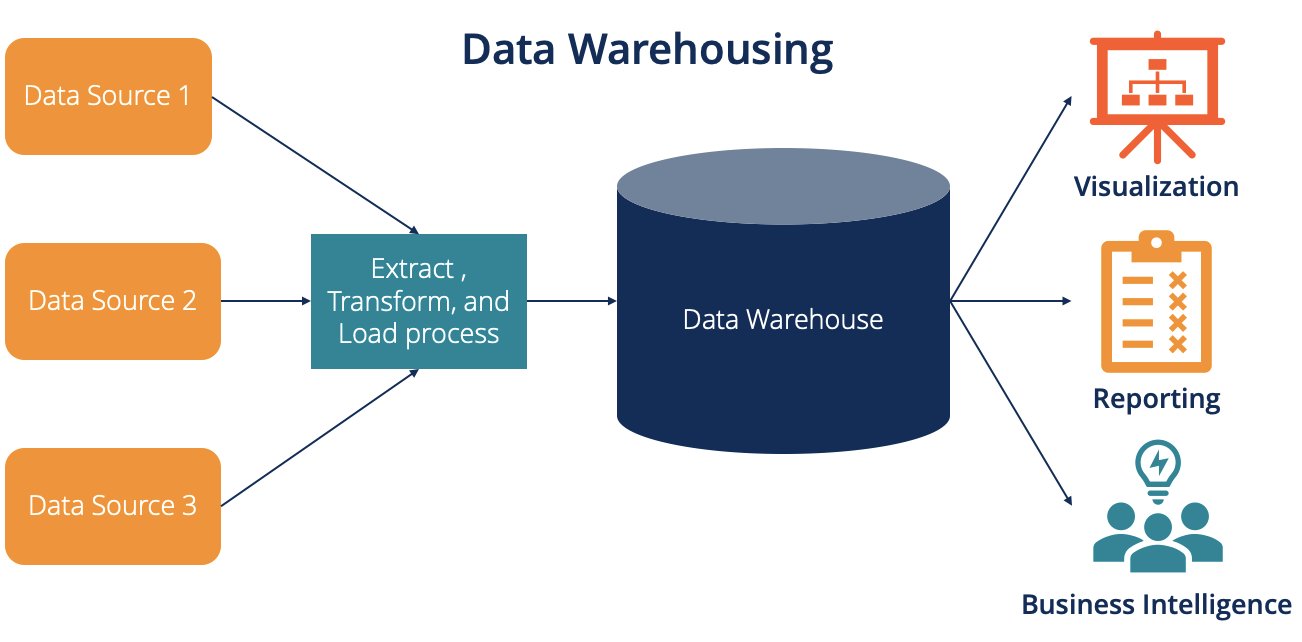
\includegraphics[width=0.8\textwidth]{data-warehouse.png}
    \caption{Representación gráfica de un Data Warehouse}
\end{figure}

Un \textit{Data Warehouse} centraliza y consolida grandes cantidades de datos provenientes de varias fuentes, como sistemas ERP, CRM, archivos de log, y más. Estos datos se procesan y transforman a través de métodos de ETL (Extracción, Transformación y Carga), que limpian los datos y los reorganizan en formatos adecuados para consultas y análisis. La finalidad de estos procesos es asegurar que los datos sean útiles y accesibles para los usuarios finales, como analistas de datos, gerentes y ejecutivos, quienes dependen de estos para realizar análisis de negocio profundizados.

Además de la operacionalización de los datos, un \textit{Data Warehouse} también facilita la implementación de soluciones de Business Intelligence (BI), como herramientas de visualización, reportes y análisis predictivo. Estas herramientas permiten a las organizaciones descubrir patrones, tendencias y obtener insights estratégicos que son cruciales para la planificación a largo plazo y la toma de decisiones efectiva.

Finalmente, un \textit{Data Warehouse} es crucial para las operaciones empresariales ya que permite a las organizaciones trabajar con datos a gran escala y extraer insights valiosos que son críticos para el desarrollo estratégico y operativo. La capacidad de un \textit{Data Warehouse} para proporcionar una visión histórica y consolidada de los datos de la empresa es inigualable, convirtiéndolo en una herramienta indispensable en el ámbito competitivo actual.

\newpage
\section*{Diseño en Modelo Estrella}
\begin{figure}[ht]
    \centering
    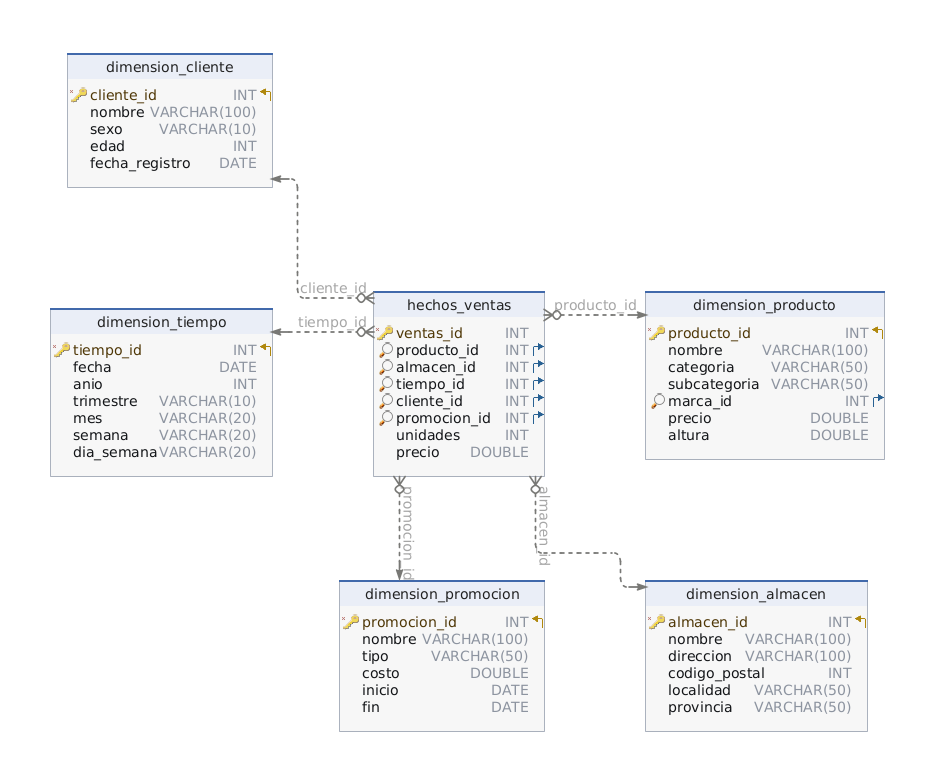
\includegraphics[width=\textwidth]{star-schema.png}
    \caption{Esquema en Estrella para Data Warehouse}
\end{figure}

\newpage
\section*{Diseño del Modelo Copo de Nieve}
\begin{figure}[ht]
    \centering
    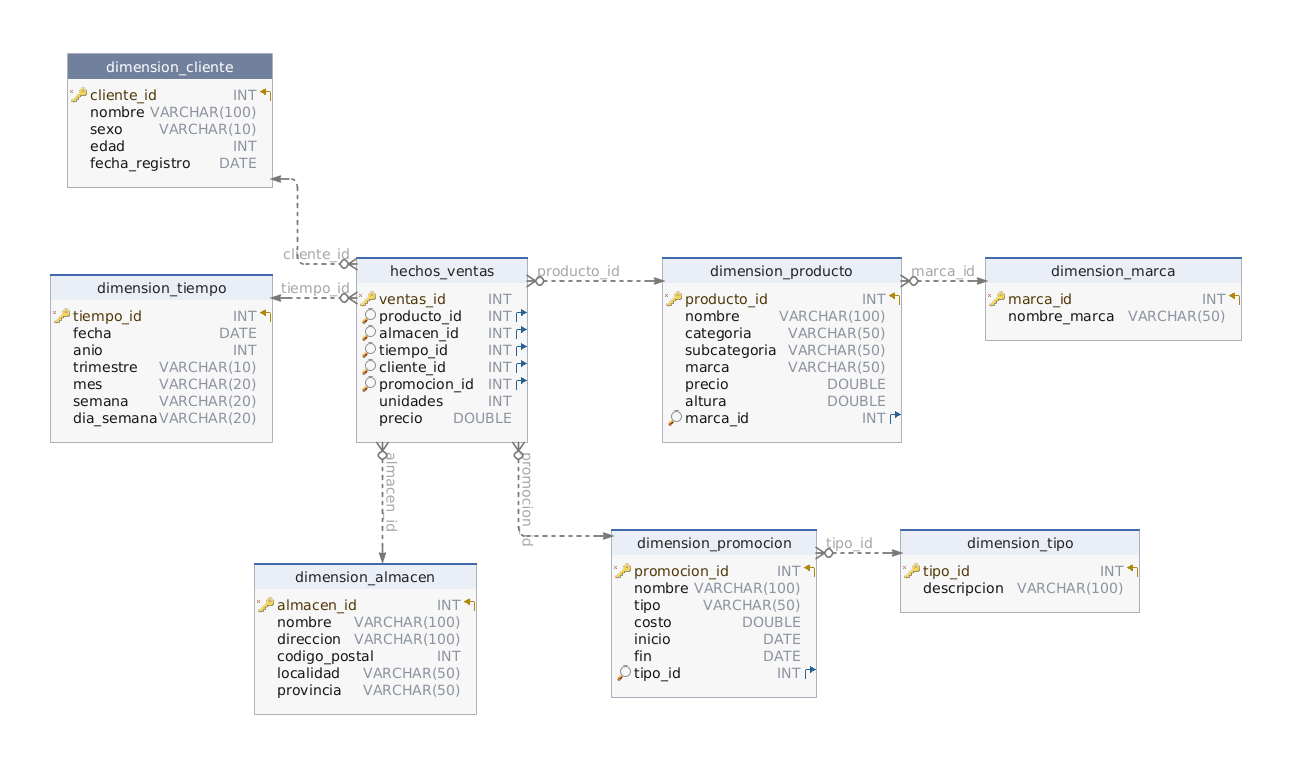
\includegraphics[width=\textwidth]{snowflake-schema.png}
    \caption{Esquema Copo de Nieve para Data Warehouse}
\end{figure}

\end{document}
